\documentclass[border=5pt]{standalone}
\usepackage{pgfplots}
\pgfplotsset{compat=1.18}
\usepackage{siunitx}
\usepackage{tikz}
\usetikzlibrary{calc}

\definecolor{adam}{RGB}{31,119,180}
\definecolor{sgd}{RGB}{255,127,14}
\definecolor{rmsprop}{RGB}{143,0,255}

\begin{document}
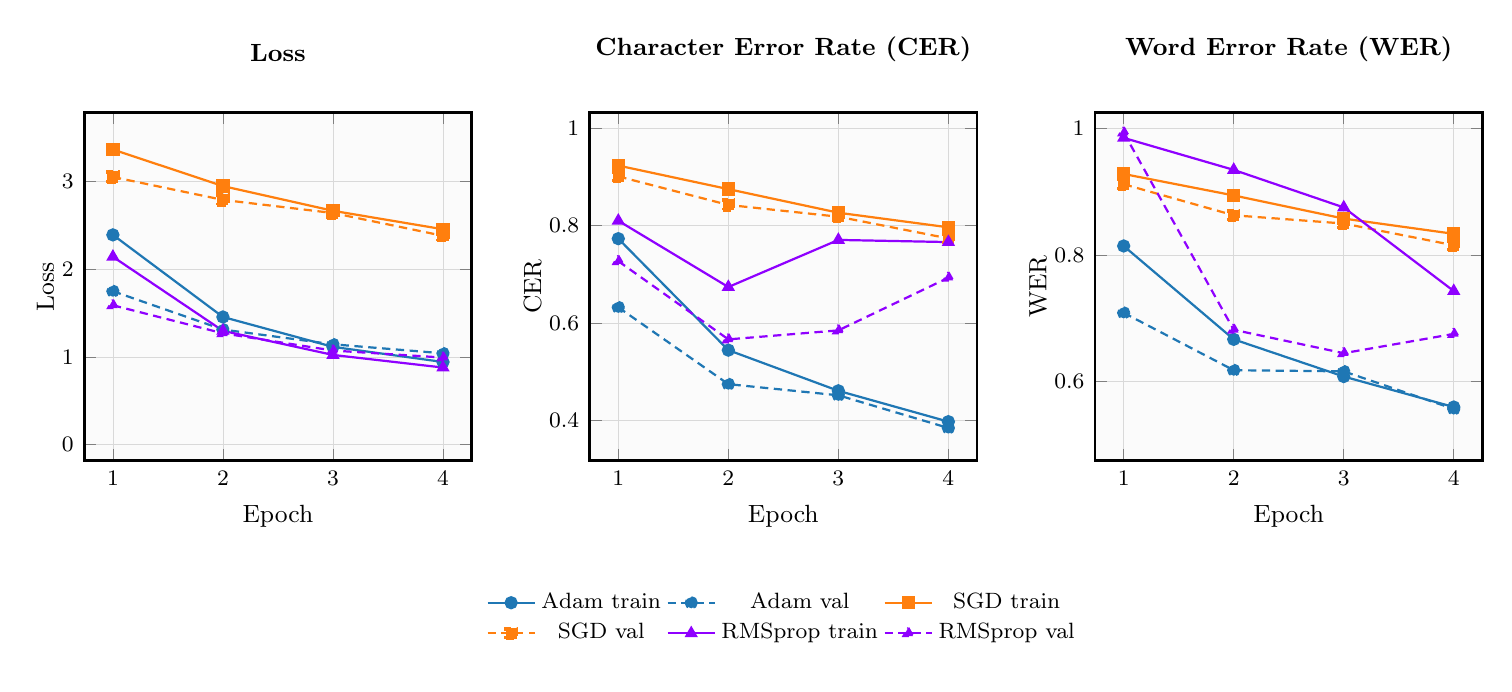
\begin{tikzpicture}[remember picture]

    % Графік 1: Loss
    \begin{axis}[
        name=plot1,
        width=6.5cm,
        height=6cm,
        xlabel={Epoch},
        ylabel={Loss},
        ylabel style={yshift=-0.15cm},
        xmin=0.9, xmax=4.1,
        ymin=0, ymax=3.6,
        xtick={1,2,3,4},
        grid=both,
        grid style={line width=.1pt, draw=gray!10},
        major grid style={line width=.2pt,draw=gray!30},
        title={Loss},
        axis background/.style={fill=gray!3},
        title style={yshift=3mm, font=\small\bfseries},
        label style={font=\small},
        tick label style={font=\footnotesize},
        line width=1pt,
        enlarge x limits=0.05,
        enlarge y limits=0.05,
        every axis plot/.append style={mark size=2pt},
        legend to name=commonlegend,
        legend columns=3,
        legend style={draw=none, fill=none, font=\footnotesize}
    ]
        % Adam
        \addplot[color=adam, mark=*, thick] coordinates {(1,2.3885) (2,1.4541) (3,1.1140) (4,0.9418)};
        \addplot[color=adam, mark=*, thick, densely dashed] coordinates {(1,1.7475) (2,1.3110) (3,1.1431) (4,1.0405)};
        
        % SGD
        \addplot[color=sgd, mark=square*, thick] coordinates {(1,3.3602) (2,2.9441) (3,2.6629) (4,2.4526)};
        \addplot[color=sgd, mark=square*, thick, densely dashed] coordinates {(1,3.0478) (2,2.7868) (3,2.6374) (4,2.3781)};
        
        % RMSprop
        \addplot[color=rmsprop, mark=triangle*, thick] coordinates {(1,2.1394) (2,1.2963) (3,1.0220) (4,0.8785)};
        \addplot[color=rmsprop, mark=triangle*, thick, densely dashed] coordinates {(1,1.5873) (2,1.2681) (3,1.0721) (4,0.9923)};
        
        \legend{Adam train, Adam val, SGD train, SGD val, RMSprop train, RMSprop val}
    \end{axis}
    
    % Графік 2: CER, розташовується праворуч від plot1
    \begin{axis}[
        name=plot2,
        at={($(plot1.east)+(1.5cm,0)$)},
        anchor=west,
        width=6.5cm,
        height=6cm,
        xlabel={Epoch},
        ylabel={CER},
        ylabel style={yshift=-0.15cm},
        xmin=0.9, xmax=4.1,
        ymin=0.35, ymax=1.0,
        xtick={1,2,3,4},
        grid=both,
        grid style={line width=.1pt, draw=gray!10},
        major grid style={line width=.2pt,draw=gray!30},
        title={Character Error Rate (CER)},
        axis background/.style={fill=gray!3},
        title style={yshift=3mm, font=\small\bfseries},
        label style={font=\small},
        tick label style={font=\footnotesize},
        line width=1pt,
        enlarge x limits=0.05,
        enlarge y limits=0.05,
        every axis plot/.append style={mark size=2pt}
    ]
        % Adam
        \addplot[color=adam, mark=*, thick] coordinates {(1,0.7735) (2,0.5444) (3,0.4608) (4,0.3974)};
        \addplot[color=adam, mark=*, thick, densely dashed] coordinates {(1,0.6324) (2,0.4745) (3,0.4516) (4,0.3844)};
        
        % SGD
        \addplot[color=sgd, mark=square*, thick] coordinates {(1,0.9237) (2,0.8753) (3,0.8268) (4,0.7968)};
        \addplot[color=sgd, mark=square*, thick, densely dashed] coordinates {(1,0.9014) (2,0.8428) (3,0.8186) (4,0.7740)};
        
        % RMSprop
        \addplot[color=rmsprop, mark=triangle*, thick] coordinates {(1,0.8103) (2,0.6741) (3,0.7709) (4,0.7665)};
        \addplot[color=rmsprop, mark=triangle*, thick, densely dashed] coordinates {(1,0.7273) (2,0.5665) (3,0.5850) (4,0.6933)};
    \end{axis}
    
    % Графік 3: WER, розташовується праворуч від plot2
    \begin{axis}[
        name=plot3,
        at={($(plot2.east)+(1.5cm,0)$)},
        anchor=west,
        width=6.5cm,
        height=6cm,
        xlabel={Epoch},
        ylabel={WER},
        ylabel style={yshift=-0.15cm},
        xmin=0.9, xmax=4.1,
        ymin=0.5, ymax=1.0,
        xtick={1,2,3,4},
        grid=both,
        grid style={line width=.1pt, draw=gray!10},
        major grid style={line width=.2pt,draw=gray!30},
        title={Word Error Rate (WER)},
        axis background/.style={fill=gray!3},
        title style={yshift=3mm, font=\small\bfseries},
        label style={font=\small},
        tick label style={font=\footnotesize},
        line width=1pt,
        enlarge x limits=0.05,
        enlarge y limits=0.05,
        every axis plot/.append style={mark size=2pt}
    ]
        % Adam
        \addplot[color=adam, mark=*, thick] coordinates {(1,0.8142) (2,0.6666) (3,0.6078) (4,0.5596)};
        \addplot[color=adam, mark=*, thick, densely dashed] coordinates {(1,0.7085) (2,0.6178) (3,0.6160) (4,0.5565)};
        
        % SGD
        \addplot[color=sgd, mark=square*, thick] coordinates {(1,0.9280) (2,0.8941) (3,0.8575) (4,0.8334)};
        \addplot[color=sgd, mark=square*, thick, densely dashed] coordinates {(1,0.9118) (2,0.8627) (3,0.8497) (4,0.8153)};
        
        % RMSprop
        \addplot[color=rmsprop, mark=triangle*, thick] coordinates {(1,0.9851) (2,0.9345) (3,0.8751) (4,0.7429)};
        \addplot[color=rmsprop, mark=triangle*, thick, densely dashed] coordinates {(1,0.9934) (2,0.6817) (3,0.6447) (4,0.6752)};
    \end{axis}

    % Розміщення загальної легенди під усіма графіками
    \node at ($(plot1.south)!0.5!(plot3.south)+(0,-2.0cm)$) {\pgfplotslegendfromname{commonlegend}};
    
\end{tikzpicture}
\end{document}